\subsection{Relativistic Heavy Ion Collider}

Πλέον ο AGS έχει πολύ μικρή ενέργεια και δεν μπορεί να συγκριθεί με τους σύγχρονους επιταχυντές. Ωστόσο, αυτό για το οποίο είναι χρήσιμος είναι το να προεπιταχύνει τις δέσμες ιόντων και πρωτονίων για τον RHIC (Εικόνα (\ref{fig2.6})). Η μεταφορά γίνεται μέσω μίας γραμμής \textit{AGS-to-RHIC Line}, στην αρχή της οποίας ο χρυσός από +77 ιονίζεται πλήρως σε +79 και στο τέλος της οι δέσμες χωρίζονται στα δύο δαχτυλίδια του RHIC, που απέχουν 90cm, με αντίθετη φορά περιστροφής.
	Η μέγιστη ενέργεια για τις συγκρούσεις ιόντων Χρυσού είναι 100GeV/n οι οποίες πραγματοποιούνται σε 6 σημεία αλληλεπίδρασης (Interaction Points - IP) και το αποτέλεσμά τους είναι η δημιουργία τόσο υψηλών θερμοκρασιών $\sim TerraK$ που εμφανίζεται μία νέα κατάσταση της ύλης στην οποία τα κουάρκ και τα γλουόνια αποδεσμεύονται από τα πρωτόνια και τα νετρόνια δημιουργώντας πλάσμα κουάρκ-γλουονίων.
	
	\begin{figure}[h!]
		\centering
		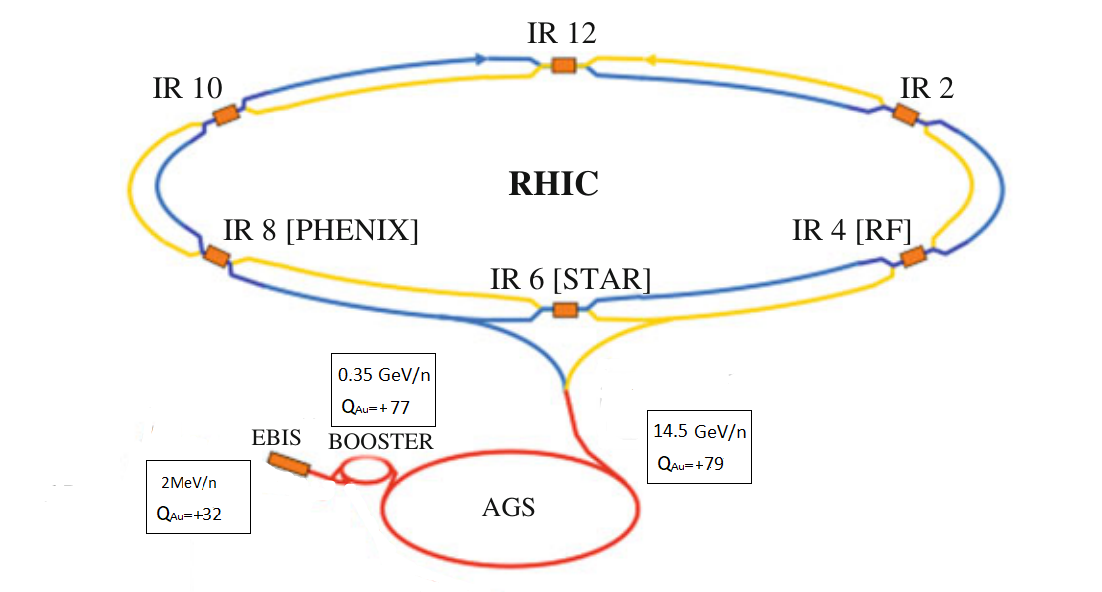
\includegraphics[scale=0.5]{Accelerating_System/RHIC_full.png}
		\caption{Τυπική πορεία των ιόντων με σημειωμένα τις τιμές φορτίου και ενέργειας του Au. }
		\label{fig2.6}
	\end{figure}
		
	
	Ο RHIC αποτελείται από 6 arc-sections μήκους 356m και από 6 insertion-sections μήκους 277m, όπως φαίνεται στην Εικόνα (\ref{fig2.7}). Στο κέντρο των τελευταίων πραγματοποιούνται οι συγκρούσεις. Τα arc-sections αποτελούνται από 11 κυψελίδες τύπου FODO με 2 διπολικούς μαγνήτες που κατευθύνουν την δέσμη, δύο τετραπολικούς οι οποίοι την εστιάζουν και δύο εξαπολικούς που επίσης την εστιάζουν με μεγαλύτερη ακρίβεια και ταυτόχρονα μειώνουν τις χρωματικές αλλοιώσεις που οφείλονται στην διασπορά της ορμής της (Ένα σχέδιο μισής περιόδου του FODO φαίνεται στην Εικόνα (\ref{fig2.8})). Επίσης, κοντά στα IP υπάρχουν επιπλέον μαγνήτες με σκοπό την γρήγορη εστιαση της δέσμης στο σημείο σύγκρουσης.	
	Συνολικά υπάρχουν 1740 υπεραγώγιμοι μαγνήτες με πεδία εως 3.458Τ.
	
	\begin{figure}[h!] 
		\centering
		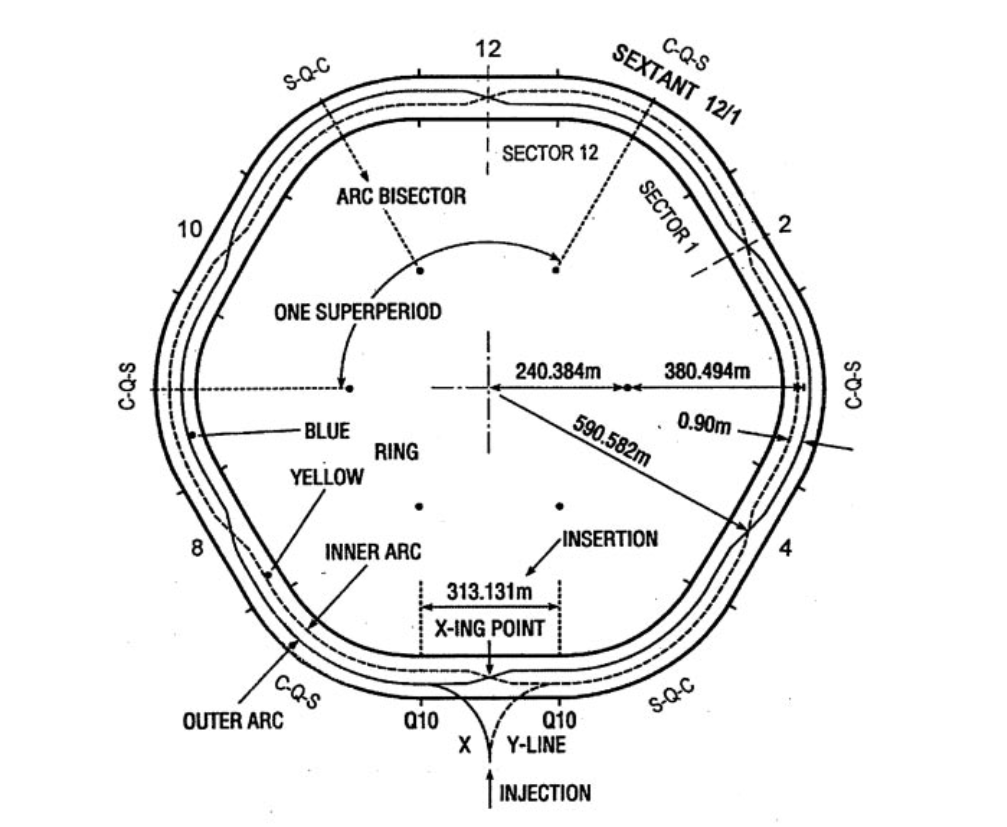
\includegraphics[scale=0.5]{Accelerating_System/RHIC_schem.png}
		\caption{Κάτοψη του RHIC }
		\label{fig2.7}
	\end{figure}
	
	
	Μία τυπική διαδικασία επιτάχυνσης αποτελείται από την εισαγωγή 111 δέσμεων σε ομάδες των 4 σε κάθε ένα από τα δύο δακτυλίδια. Αρχικά, επειδή η ενέργειά τους δεν είναι η μέγιστη,  οι δέσμες στα Interaction Points απέχουν 10mm για να αποφευγχθούν ανεπιθύμητες απώλειες και όταν φτάσουν στην μέγιστη ενέργεια, οι δέσμες συγκρούονται μετωπικά. 
	
	\begin{figure}[h!]
		\centering 
		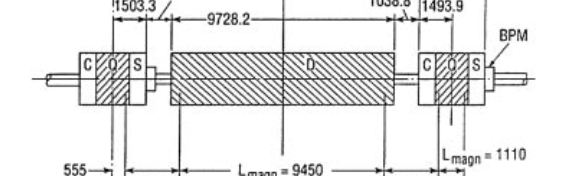
\includegraphics[scale=0.5]{Accelerating_System/RHIC_half_cells.png}
		\caption{ Σχέδιο μισής περιόδου ενός FODO του RHIC}
		\label{fig2.8}
	\end{figure}
	
	
	Όταν φτάσουν σε αυτό το σημείο μέγιστης ενέργειας, τότε ο RHIC λειτουργεί ως Storage Ring. Ο αριθμός των σωματιδίων στην δέσμη είναι πολύ μικρός ($10^9-10^{10}$ ανά bunch) και ως εκτούτου η πιθανότητα αλληλεπίδρασης είναι επίσης μικρή, πόσο μάλλον οι ισχυρές συγκούσεις που απαιτούνται για την δημιουργία των πιό ενδιαφέροντων γεγονότων. Αυτό σημαίνει ότι για να επιτευγχθούν τα απαραίτητα γεγονότα θα πρέπει να διατηρηθεί η δέσμη αρκετές ώρες (έως 10) εντός του RHIC. 
	Ο αριθμός γεγονότων ανά δευτερόλεπτο δίνεται από την σχέση 
		\begin{align*}\label{eq2.7}
			N_p = \sigma_p \mathcal{L} \numberthis
		\end{align*}	
	Όπου $\sigma_p$ είναι η ενεργός διατομή της αλληλεπίδρασης Au-Au και $\mathcal{L}$ είναι η φωτεινότητα της δέσμης. Αυτό σημαίνει πως ο μόνος τρόπος για να αυξήσουμε τον αριθμό αλληλεπιδράσεων, δεδομένου ότι η ενεργός διατομή είναι εγγενές χαρακτηριστικό της εκάστοτε αλληλεπίδρασης, είναι η αύξηση της φωτεινότητας.
		\textcolor{red}{ΛΙΓΑ ΛΟΓΙΑ ΓΙΑ ΛΟΥΜΙΝΟΣΙΤΙ}	
		Η φωτεινότητα είναι ο λόγος των γεγονότων σε ένα χρονικό διάστημα ανά ενεργό διατομή, δηλαδή ορίζεται από την σχέση $\mathcal{L} = (1/\sigma)dN/dt$ και έχει μονάδες $[cm^{-2}s^{-1}]$. Για έναν collider όπως ο RHIC, υπολογίζεται από την σχέση
			\begin{align}\label{eq2.8}
				\mathcal{L} = \frac{1}{4\pi}\frac{fN_1N_2}{\sigma_x\sigma_y}
			\end{align}
	όπου f συχνότητα περιστροφής των σωματιδίων, $N_1, N_2$ ο αριθμός σωματιδίων σε κάθε δέσμη και $\sigma_x\sigma_y$ η διατομή της δέσμης κάθετα στο επίπεδο κίνησης. Άρα από τα παραπάνω προκύπτει κάτι που είναι και διαισθητικά αναμενόμενο, δηλαδή ότι ο αριθμός των συγκρούσεων αυξάνεται καθώς αυξάνεται η συχνότητα περιστροφής των σωματιδίων, ο αριθμός των σωματιδίων και καθώς εστιάζεται περισσότερο η δέσμη. Στον RHIC η μέση φωτεινότητα είναι $20\times10^{26}cm^{-2}s^{-1}$ για τις συγκρούσεις Au-Au ενώ η μέγιστη δυνατή που επιτυγχάνεται στα IP, σε μία εκ των οποίων  βρίσκεται και το πείραμα STAR, είναι $40\times10^{26}cm^{-2}s^{-1}$
		
		
	
	
	
